\section{Results}
\label{sec:results}

We first report rank curves at a fixed learning rate (\secref{sec:res_curves}) and the cost of $r{=}8$ (\secref{sec:res_gap}). We then show that the learning rate explains most of the rank effect (\secref{sec:res_lr}), and we close with model size (\secref{sec:res_size}) and the gradient predictor (\secref{sec:res_pred}).

\subsection{Rank curves at a fixed learning rate}
\label{sec:res_curves}

\begin{table}[t]
    \centering
    \caption{Evaluation metric (\%) vs.\ \lora rank at learning rate $2\times10^{-4}$. 0.5B values are the mean of 2 seeds (seed SD $\leq$1.3\pp except \boolq $r{=}128$, 5.7\pp); 1.5B values use 1 seed. $r{=}0$ is the zero-shot base model. The best adapter rank per row is in {\bf bold}. Classification curves are flat after $r{=}8$, \emotion keeps rising, and \gsm and code peak at low rank.}
    \label{tab:rank_grid}
    \resizebox{\textwidth}{!}{%
    \begin{tabular}{@{}llccccccccc@{}}
        \toprule
        & & \multicolumn{1}{c}{\textbf{Zero-shot}} & \multicolumn{8}{c}{\textbf{\lora rank $r$}} \\
        \cmidrule(lr){3-3} \cmidrule(lr){4-11}
        \textbf{Model} & \textbf{Task} & $r{=}0$ & 1 & 2 & 4 & 8 & 16 & 32 & 64 & 128 \\
        \midrule
        \multirow{6}{*}{0.5B}
        & \sst     & 88.5 & 91.7 & 91.7 & 92.4 & 92.8 & 92.9 & {\bf 93.3} & 92.5 & 91.5 \\
        & \emotion & 52.6 & 77.7 & 81.6 & 86.3 & 89.7 & 91.2 & 91.7 & 92.1 & {\bf 92.3} \\
        & \agnews  & 75.9 & 89.3 & 89.7 & 90.1 & 90.7 & 90.7 & 91.0 & {\bf 91.1} & 90.4 \\
        & \boolq   & 62.9 & 74.2 & 74.4 & 74.9 & 76.4 & 77.3 & {\bf 78.0} & 76.5 & 67.1 \\
        & \gsm     & 3.4  & {\bf 37.3} & 34.8 & 35.4 & 34.1 & 33.4 & 33.0 & 32.3 & 30.1 \\
        & \code    & 27.0 & 27.8 & 28.4 & 27.9 & 27.7 & {\bf 28.8} & 27.6 & 24.5 & 22.7 \\
        \midrule
        \multirow{6}{*}{1.5B}
        & \sst     & 54.2 & 95.0 & 95.1 & 95.0 & 95.3 & {\bf 95.6} & 95.4 & 94.7 & 94.5 \\
        & \emotion & 52.6 & 79.1 & 82.2 & 87.1 & 91.0 & 92.6 & {\bf 93.2} & 92.9 & 92.3 \\
        & \agnews  & 77.8 & 90.1 & 89.8 & 90.1 & 90.8 & 90.7 & 91.4 & 90.8 & {\bf 91.5} \\
        & \boolq   & 67.6 & 81.6 & 82.9 & 83.7 & 84.4 & 84.4 & 84.3 & {\bf 85.5} & 83.0 \\
        & \gsm     & 9.6  & 58.8 & 58.2 & 60.0 & 60.0 & 59.6 & {\bf 60.6} & 58.2 & 55.0 \\
        & \code    & 47.2 & {\bf 46.2} & 45.2 & 44.8 & 44.0 & 45.0 & 44.0 & 42.8 & 40.6 \\
        \bottomrule
    \end{tabular}}
\end{table}


\begin{figure}[t]
    \centering
    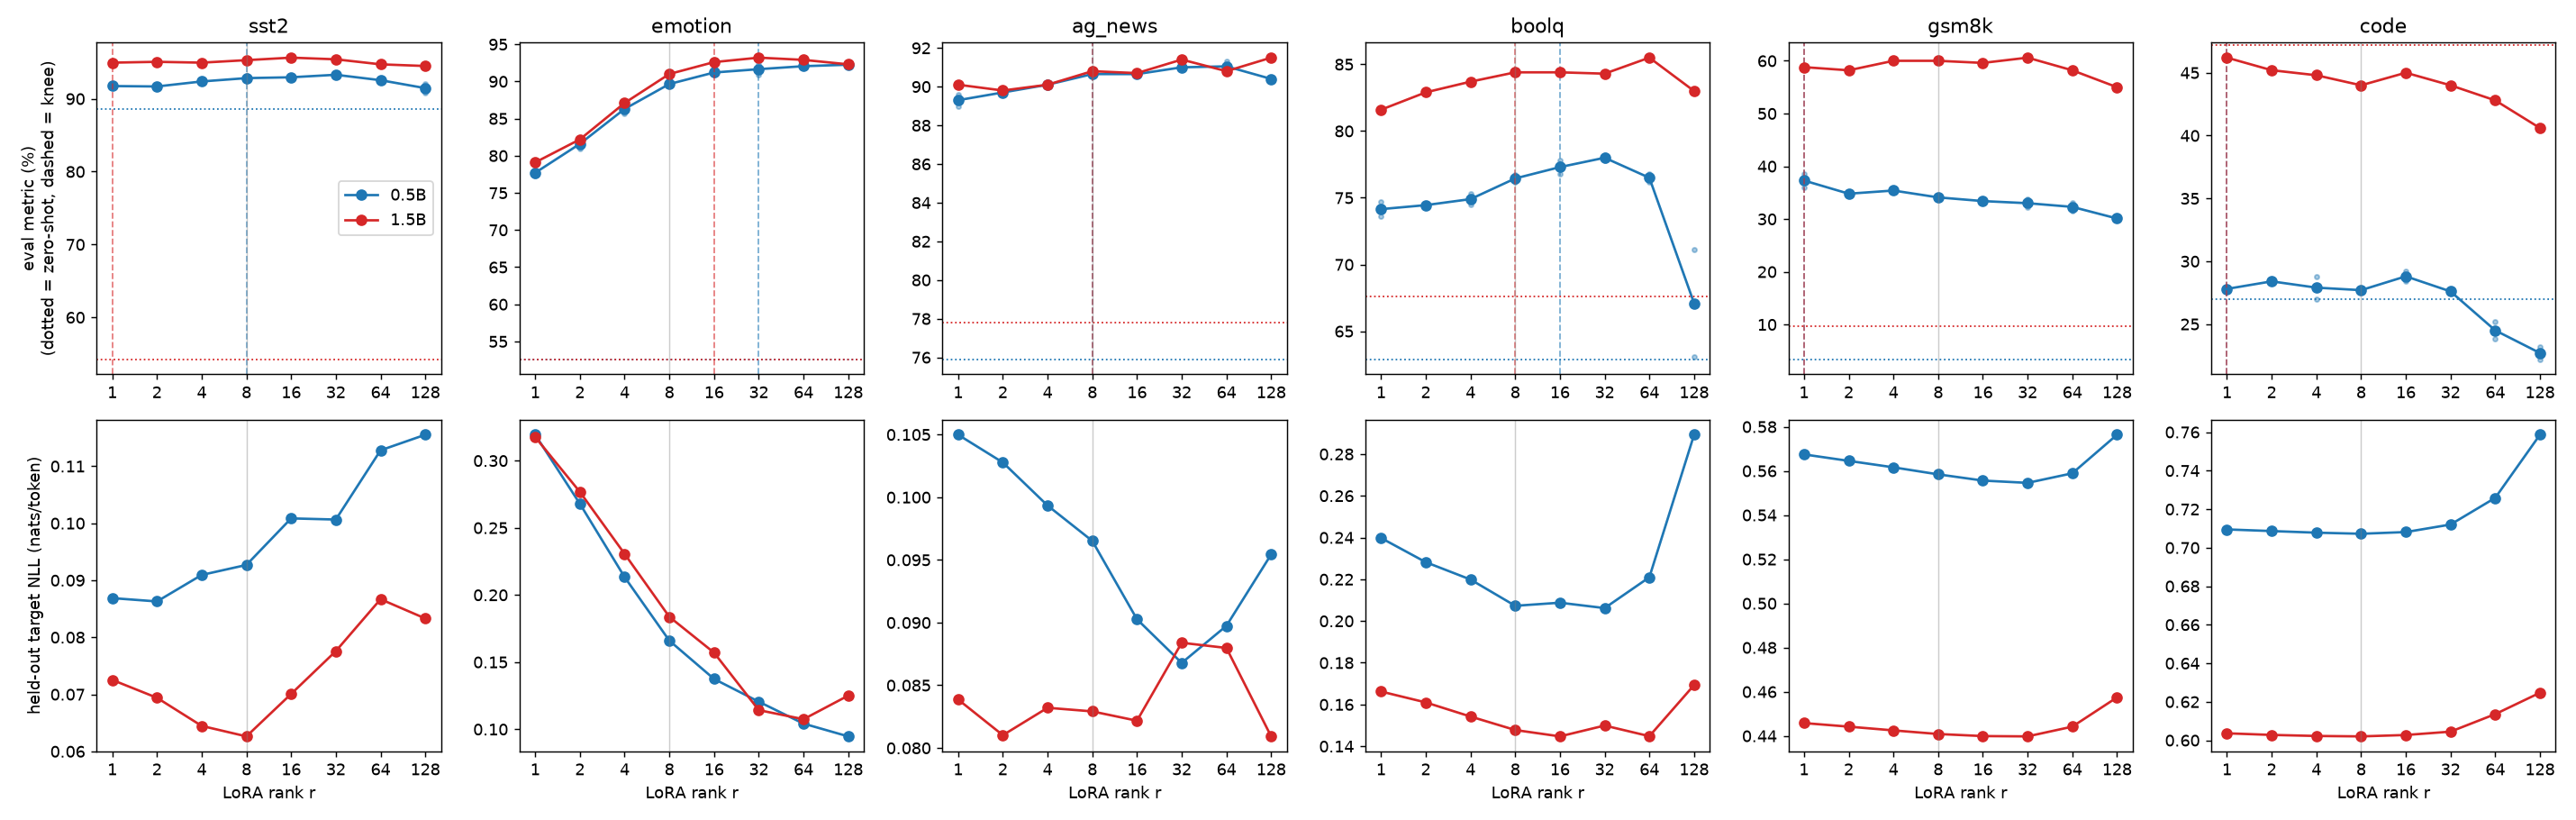
\includegraphics[width=\linewidth]{figures/rank_curves.png}
    \caption{Rank curves at learning rate $2\times10^{-4}$. \figtop\ Evaluation metric vs.\ \lora rank (lines are seed means, faint dots are individual seeds, dotted lines are zero-shot, dashed vertical lines are knees, grey line marks $r{=}8$). \figbottom\ Held-out target NLL. Only \emotion has a steep, monotone rank curve. \gsm and code decline with rank, and their NLL worsens at $r\geq64$. Curve shapes are nearly identical for 0.5B (blue) and 1.5B (red).}
    \label{fig:rank_curves}
\end{figure}

\Tabref{tab:rank_grid} and \figref{fig:rank_curves} show the main grid. {\bf Does the best rank vary across tasks?} Yes: it ranges from $r{=}1$ (0.5B \gsm, 1.5B code) to $r{=}128$ (0.5B \emotion, 1.5B \agnews). But the task ordering is not the one the folk wisdom predicts.

\para{Classification is flat.} On \sst and \agnews, $r{=}1$ is already within 1.3\pp of the best rank for 0.5B, and the curve barely moves after $r{=}8$.

\para{Emotion is the one steep curve.} 6-way \emotion rises from 77.7\% at $r{=}1$ to 89.7\% at $r{=}8$ and 92.3\% at $r{=}128$ on 0.5B. 1.5B follows the same shape.

\para{Math and code prefer low rank.} \gsm accuracy falls almost monotonically with rank on 0.5B: 37.3\% at $r{=}1$, 34.1\% at $r{=}8$, and 30.1\% at $r{=}128$. Held-out NLL stays nearly flat (0.555--0.568) up to $r{=}64$ and then worsens. On \code, fine-tuning barely beats zero-shot on 0.5B (best 28.8\% at $r{=}16$ vs.\ 27.0\%), and $r{=}128$ drops to 22.7\%, below zero-shot. On 1.5B, every code adapter scores below the 47.2\% zero-shot pass@1.

\para{Large ranks can collapse.} \boolq rises to 78.0\% at $r{=}32$ and then drops to 67.1\% at $r{=}128$ (seeds: 63.1\% and 71.1\%). Together with \gsm and code, large ranks at the default learning rate cost 7--11\pp on three of six tasks for 0.5B.

\subsection{How much does $r{=}8$ cost?}
\label{sec:res_gap}

\begin{table}[t]
    \centering
    \caption{Knee ranks and the cost of the $r{=}8$ default at learning rate $2\times10^{-4}$. Gap = best $-$ $r{=}8$ (pp), with a paired-bootstrap 95\% CI over evaluation items. ``Best $r{>}8$'' is the gain of the best rank above 8 over $r{=}8$. Cross-fitted gaps choose the best rank on one seed and score it on the other (0.5B only). $p_\text{Holm}$ is Holm-adjusted over tasks. Rows with $p_\text{Holm}<0.05$ are in {\bf bold}. Only \emotion gains significantly from a rank above 8. The \gsm and 1.5B code gaps favour $r{=}1$, \ie a rank \emph{smaller} than 8.}
    \label{tab:gap}
    \resizebox{\textwidth}{!}{%
    \begin{tabular}{@{}llcccccccc@{}}
        \toprule
        \textbf{Model} & \textbf{Task} & \textbf{Best $r$} & \textbf{Knee} & \textbf{NLL knee} & \textbf{Gap (pp)} & \textbf{95\% CI} & \textbf{Cross-fit} & \textbf{Best $r{>}8$ $-$ $r8$} & $p_\text{Holm}$ \\
        \midrule
        \multirow{6}{*}{0.5B}
        & \sst     & 32  & 8  & 1 & 0.5 & [$-$0.5, 1.4] & 0.5 & 0.5 & 1.0 \\
        & {\bf \emotion} & {\bf 128} & {\bf 32} & {\bf 1} & {\bf 2.6} & {\bf [1.2, 4.0]} & {\bf 1.8} & {\bf 2.6} & {\bf $<$0.001} \\
        & \agnews  & 64  & 8  & 1 & 0.4 & [$-$0.4, 1.1] & 0.3 & 0.4 & 1.0 \\
        & \boolq   & 32  & 16 & 2 & 1.6 & [$-$0.1, 3.1] & 0.9 & 1.6 & 0.454 \\
        & \gsm     & 1   & 1  & 1 & 3.2 & [0.7, 5.7]    & 3.2 & $-$0.7 & 0.132 \\
        & \code    & 16  & 1  & 2 & 1.1 & [$-$0.3, 2.5] & 0.7 & 1.1 & 0.89 \\
        \midrule
        \multirow{6}{*}{1.5B}
        & \sst     & 16  & 1  & 1 & 0.3 & [$-$0.5, 1.3] & -- & 0.3 & 1.0 \\
        & {\bf \emotion} & {\bf 32} & {\bf 16} & {\bf 1} & {\bf 2.2} & {\bf [0.8, 3.6]} & -- & {\bf 2.2} & {\bf 0.018} \\
        & \agnews  & 128 & 8  & 1 & 0.7 & [$-$0.5, 1.9] & -- & 0.7 & 1.0 \\
        & \boolq   & 64  & 8  & 1 & 1.1 & [$-$0.6, 2.8] & -- & 1.1 & 1.0 \\
        & \gsm     & 32  & 1  & 1 & 0.6 & [$-$2.6, 3.8] & -- & 0.6 & 1.0 \\
        & \code    & 1   & 1  & 1 & 2.2 & [0.2, 4.2]    & -- & 1.0 & 0.324 \\
        \bottomrule
    \end{tabular}}
\end{table}


\Tabref{tab:gap} tests the rank-8 gap. {\bf H1 (rank needs vary $\geq 8\times$)} holds numerically: knees range from 1 to 32. However, the direction is reversed. \gsm and code have the \emph{lowest} knees ($r{=}1$ for both models), and \emotion has the highest ($r{=}32$ for 0.5B, $r{=}16$ for 1.5B).

{\bf H2 ($r{=}8$ costs 3--8\pp on high-rank tasks)} is not supported. The largest gain from any rank above 8 is $+2.6$\pp on 0.5B \emotion (CI [1.2, 4.0], $p_\text{Holm}<0.001$). It shrinks to $+1.8$\pp when cross-fitted across seeds, which removes the winner's-curse bias. On 1.5B \emotion the gain is $+2.2$\pp ($p_\text{Holm}=0.018$). These are the only significant gaps after correction. No generative task gains more than 1\pp from a rank above 8. On 0.5B \gsm the best rank above 8 is 0.7\pp \emph{worse} than $r{=}8$. The two largest uncorrected gaps, 0.5B \gsm ($+3.2$\pp, CI [0.7, 5.7]) and 1.5B code ($+2.2$\pp, CI [0.2, 4.2]), both favour $r{=}1$. On these tasks, $r{=}8$ is too large, not too small.

\subsection{The rank effect is mostly a learning-rate effect}
\label{sec:res_lr}

\begin{table}[t]
    \centering
    \caption{Rank $\times$ learning-rate sweep on \qsmall (seed 0). Metric in \%. The best value in each (task, rank) column is in {\bf bold}. ``Best over lr'' takes the per-rank maximum. With a tuned learning rate, the spread across ranks is 0.7\pp on \emotion, 1.8\pp on \code, and 3.6\pp on \gsm (favouring $r{=}8$ over $r{=}128$).}
    \label{tab:lr}
    \small
    \begin{tabular}{@{}lcccc@{\hskip 14pt}cccc@{\hskip 14pt}cccc@{}}
        \toprule
        & \multicolumn{4}{c}{\textbf{\emotion}} & \multicolumn{4}{c}{\textbf{\gsm}} & \multicolumn{4}{c}{\textbf{\code}} \\
        \cmidrule(lr){2-5} \cmidrule(lr){6-9} \cmidrule(lr){10-13}
        \textbf{lr} & $r2$ & $r8$ & $r32$ & $r128$ & $r2$ & $r8$ & $r32$ & $r128$ & $r2$ & $r8$ & $r32$ & $r128$ \\
        \midrule
        $2\times10^{-5}$ & -- & -- & -- & -- & -- & 36.2 & -- & {\bf 34.0} & -- & 28.4 & -- & {\bf 27.8} \\
        $5\times10^{-5}$ & 68.9 & 77.5 & 87.0 & 92.1 & 35.8 & {\bf 37.6} & {\bf 35.0} & 30.2 & 28.6 & 28.4 & {\bf 29.6} & {\bf 27.8} \\
        $1\times10^{-4}$ & 74.7 & 84.8 & 91.0 & {\bf 92.4} & {\bf 36.0} & 35.6 & 33.0 & 33.0 & {\bf 29.0} & {\bf 28.8} & 28.6 & 25.2 \\
        $2\times10^{-4}$ & 82.2 & 89.6 & {\bf 92.4} & {\bf 92.4} & 35.2 & 34.0 & 32.2 & 30.0 & 28.4 & 27.8 & 27.6 & 22.2 \\
        $5\times10^{-4}$ & 90.3 & {\bf 92.8} & {\bf 92.4} & 90.5 & 35.0 & 32.2 & 31.2 & 22.4 & {\bf 29.0} & 26.6 & 22.8 & 15.4 \\
        $1\times10^{-3}$ & {\bf 92.1} & {\bf 92.8} & -- & -- & -- & -- & -- & -- & -- & -- & -- & -- \\
        $2\times10^{-3}$ & 91.7 & 91.0 & -- & -- & -- & -- & -- & -- & -- & -- & -- & -- \\
        \midrule
        Best over lr & 92.1 & 92.8 & 92.4 & 92.4 & 36.0 & 37.6 & 35.0 & 34.0 & 29.0 & 28.8 & 29.6 & 27.8 \\
        \bottomrule
    \end{tabular}
\end{table}


\begin{figure}[t]
    \centering
    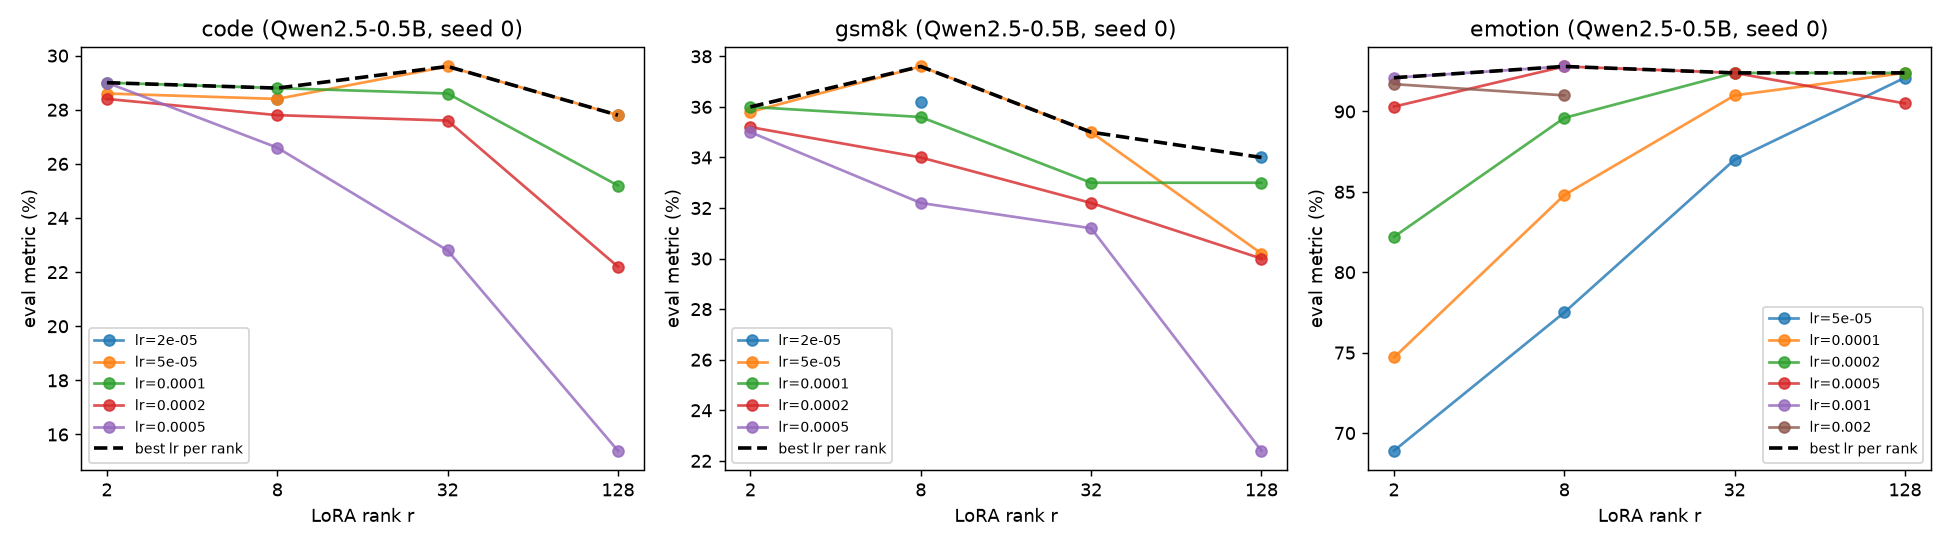
\includegraphics[width=\linewidth]{figures/lr_sweep.png}
    \caption{Metric vs.\ rank for each learning rate on \qsmall (seed 0). The dashed black line takes the best learning rate per rank. \figright\ On \emotion, low learning rates produce a steep ``needs high rank'' curve, while learning rates of $5\times10^{-4}$--$10^{-3}$ give a flat curve. \figleft\ and \figcenter\ On \code and \gsm, high rank never helps, and high rank combined with a high learning rate is destructive.}
    \label{fig:lr_sweep}
\end{figure}

\Tabref{tab:lr} and \figref{fig:lr_sweep} show the rank $\times$ learning-rate sweep. {\bf Does the \emotion gap survive learning-rate tuning?} No. At learning rate $5\times10^{-5}$, \emotion accuracy climbs from 68.9\% ($r{=}2$) to 92.1\% ($r{=}128$), a textbook ``needs high rank'' curve. At $5\times10^{-4}$--$10^{-3}$ the curve is flat: 92.1\% ($r{=}2$), 92.8\% ($r{=}8$), 92.4\% ($r{=}32$), 92.4\% ($r{=}128$). The best-over-lr spread across ranks is only 0.7\pp, and $r{=}8$ is the best rank. By contrast, the learning rate changes $r{=}8$ accuracy by 15.3\pp (77.5\% to 92.8\%). The explanation is the $\alpha=2r$ scaling: the update $2\mB\mA$ is a sum of $r$ rank-1 terms trained at the same learning rate, so a larger rank acts like a larger step. A low rank at a higher learning rate reaches the same accuracy.

On \gsm, the best-over-lr accuracy is highest at $r{=}8$ (37.6\%, learning rate $5\times10^{-5}$) and lowest at $r{=}128$ (34.0\%, $2\times10^{-5}$). High rank never helps, and at a high learning rate it is destructive ($r{=}128$ at $5\times10^{-4}$: 22.4\%). On \code, best-over-lr pass@1 is flat (27.8--29.6\%) and within noise (SE $\approx$ 2\pp). $r{=}128$ at $5\times10^{-4}$ falls to 15.4\%, with held-out NLL rising from 0.708 to 0.857.

The best learning rate shrinks as rank grows on all three tasks: on \emotion from $10^{-3}$ ($r{=}2$) to $10^{-4}$--$2\times10^{-4}$ ($r{=}128$), on \gsm from $10^{-4}$ to $2\times10^{-5}$, and on \code from $10^{-4}$/$5\times10^{-4}$ to $2\times10^{-5}$/$5\times10^{-5}$. This is the coupling expected under $\alpha\propto r$. The common recipe of ``$r{=}8$ with learning rate $2\times10^{-4}$'' is a matched pair. Changing the rank without changing the learning rate creates apparent rank effects.

\subsection{Does the knee shrink with model size?}
\label{sec:res_size}

\begin{table}[t]
    \centering
    \caption{Effect of model size at learning rate $2\times10^{-4}$. The knee is lower for 1.5B on 3 tasks, equal on 3, and never higher (sign test $p=0.25$). The clearest size effect is robustness to large ranks: on \boolq, $r{=}128$ costs 10.9\pp at 0.5B but 2.5\pp at 1.5B.}
    \label{tab:size}
    \small
    \begin{tabular}{@{}lcccccc@{}}
        \toprule
        & \multicolumn{2}{c}{\textbf{Knee}} & \multicolumn{2}{c}{\textbf{Best rank}} & \multicolumn{2}{c}{\textbf{$r128 -$ best (pp)}} \\
        \cmidrule(lr){2-3} \cmidrule(lr){4-5} \cmidrule(lr){6-7}
        \textbf{Task} & 0.5B & 1.5B & 0.5B & 1.5B & 0.5B & 1.5B \\
        \midrule
        \sst     & 8  & {\bf 1}  & 32  & 16  & $-$1.8  & $-$1.1 \\
        \emotion & 32 & {\bf 16} & 128 & 32  & 0.0     & $-$0.9 \\
        \agnews  & 8  & 8        & 64  & 128 & $-$0.7  & 0.0 \\
        \boolq   & 16 & {\bf 8}  & 32  & 64  & $-$10.9 & $-$2.5 \\
        \gsm     & 1  & 1        & 1   & 32  & $-$7.2  & $-$5.6 \\
        \code    & 1  & 1        & 16  & 1   & $-$6.1  & $-$5.6 \\
        \bottomrule
    \end{tabular}
\end{table}


\Tabref{tab:size} compares the two model sizes. {\bf H3} is directionally consistent but not statistically supported. The knee is lower for 1.5B on \sst, \emotion, and \boolq, equal on the other three tasks, and never higher. A sign test on the three non-tied pairs gives $p=0.25$. The best rank moves in both directions. The fixed-learning-rate curves have nearly the same shape at both sizes (\figref{fig:rank_curves}). The clearest size effect is robustness: 1.5B suffers much less from the $r{=}128$ collapse on \boolq ($-2.5$\pp vs.\ $-10.9$\pp).

\subsection{Does the initial gradient spectrum predict rank needs?}
\label{sec:res_pred}

\begin{table}[t]
    \centering
    \caption{Gradient spectrum statistics at initialization (median over target matrices). \rninety, $r_{99}$: directions needed for 90\% / 99\% of gradient energy. \erank: entropy effective rank. Top-8: fraction of energy in the top 8 directions. The ordering code $\gg$ \gsm $>$ \boolq $>$ \agnews $>$ \emotion $>$ \sst is consistent across sizes.}
    \label{tab:gradid}
    \small
    \begin{tabular}{@{}lccccccc@{}}
        \toprule
        & \multicolumn{4}{c}{\textbf{\qsmall}} & \multicolumn{3}{c}{\textbf{\qlarge}} \\
        \cmidrule(lr){2-5} \cmidrule(lr){6-8}
        \textbf{Task} & \rninety & $r_{99}$ & \erank & Top-8 & \rninety & $r_{99}$ & \erank \\
        \midrule
        \sst     & 2 & 4   & 7.4   & 0.999 & 2 & 5   & 10.2 \\
        \emotion & 2 & 5   & 10.3  & 0.999 & 2 & 5   & 12.3 \\
        \agnews  & 2 & 5   & 17.0  & 0.997 & 2 & 5   & 18.6 \\
        \boolq   & 2 & 7   & 26.1  & 0.993 & 2 & 6.5 & 22.4 \\
        \gsm     & 4 & 9   & 46.3  & 0.990 & 4 & 11  & 80.4 \\
        \code    & 6 & 143 & 223.7 & 0.919 & 3 & 89  & 244.2 \\
        \bottomrule
    \end{tabular}
\end{table}


\begin{figure}[t]
    \centering
    \begin{subfigure}[b]{0.8\textwidth}
        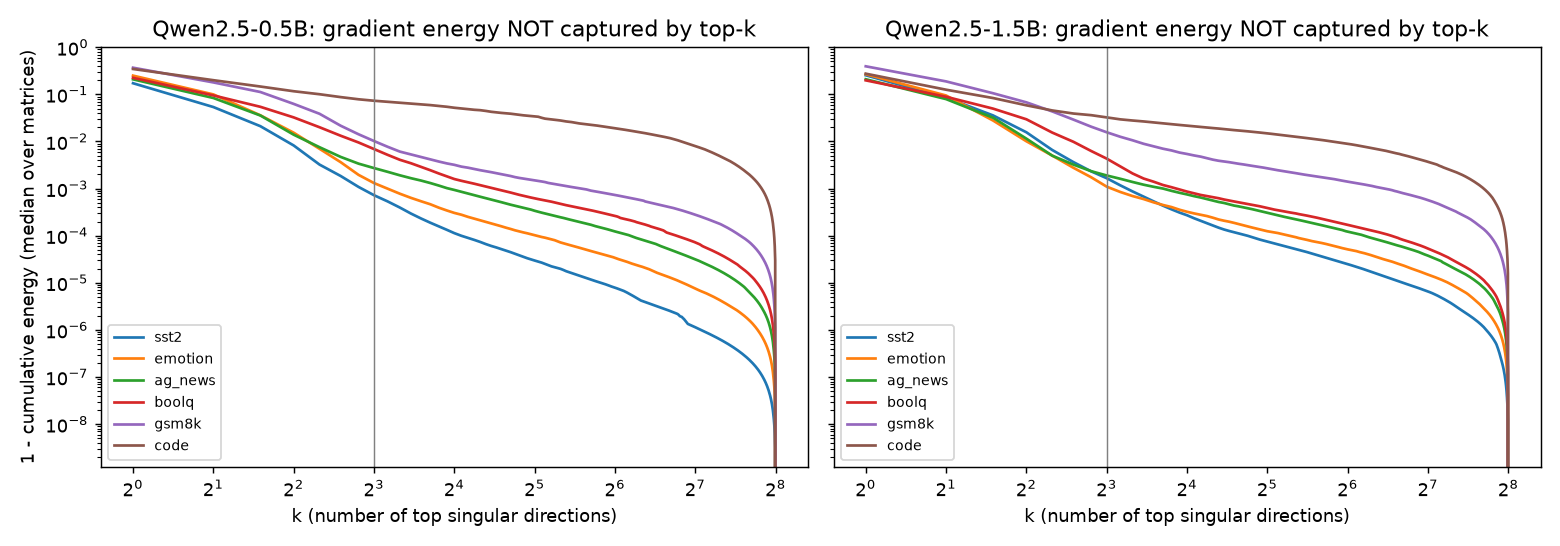
\includegraphics[width=\textwidth]{figures/gradient_spectra.png}
        \caption{Gradient energy outside the top-$k$ directions}
        \label{fig:spectra}
    \end{subfigure}
    \\[4pt]
    \begin{subfigure}[b]{0.95\textwidth}
        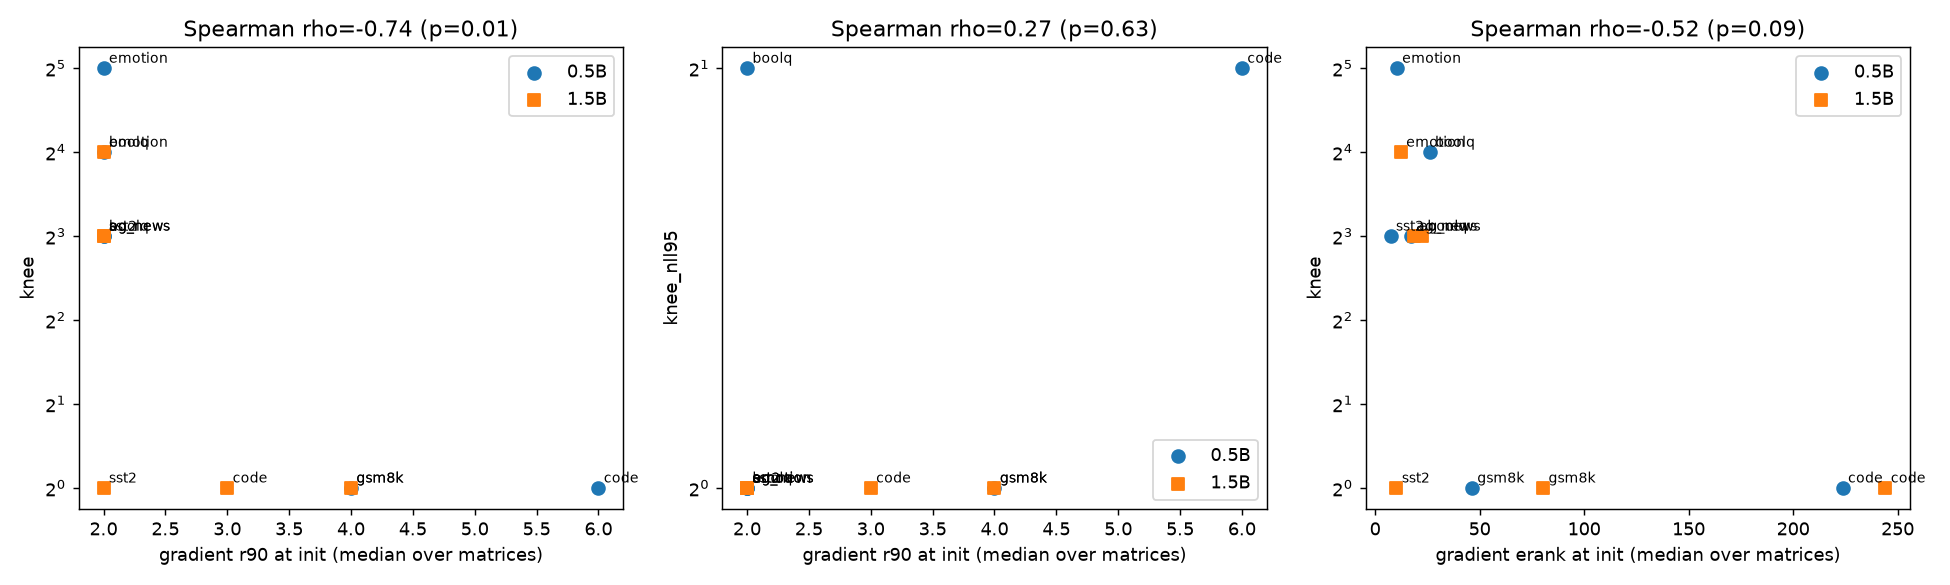
\includegraphics[width=\textwidth]{figures/gradid_vs_knee.png}
        \caption{Gradient statistic vs.\ empirical knee}
        \label{fig:gradid_knee}
    \end{subfigure}
    \caption{The gradient-spectrum predictor. \captiona\ Fraction of gradient energy not captured by the top-$k$ singular directions, median over target matrices, for 0.5B (left) and 1.5B (right). Spectra are truncated at 256, so curves drop to 0 there by construction. The grey line marks $k{=}8$. Code has by far the heaviest tail. \captionb\ \rninety (left), \rninety vs.\ NLL knee (middle), and \erank (right) against the knee rank (log scale). Tasks with the heaviest gradient tails (code, \gsm) have the \emph{lowest} knees.}
    \label{fig:gradid}
\end{figure}

\Tabref{tab:gradid} and \figref{fig:spectra} show that the gradient statistic separates tasks cleanly and consistently across model sizes. The code gradient spreads over two orders of magnitude more directions than \sst (\erank 223.7 vs.\ 7.4 on 0.5B), and only 91.9\% of its energy lies in the top 8 directions, compared with 99.9\% for \sst.

{\bf H4 (the statistic predicts the knee with $\rho>0.7$)} is refuted, with a significant correlation of the opposite sign (\tabref{tab:predictor}, \figref{fig:gradid_knee}). The primary predictor \rninety has $\rho=-0.74$ ($p=0.014$) with the knee. All other gradient statistics also correlate negatively ($\rho$ from $-0.52$ to $-0.63$). With a leave-one-out calibrated scale, \rninety lands within $2\times$ of the knee for 0 of 12 pairs, while always predicting $r{=}8$ succeeds for 6 of 12. The NLL knee shows a weak positive correlation ($\rho=0.27$, $p=0.63$). Its high hit rate (0.92) is not informative, because NLL knees are 1 or 2 for every pair.

\begin{table}[t]
    \centering
    \caption{How well initial-gradient statistics predict rank needs over $n=12$ (task, model) pairs. Positive $\rho$ means ``predicts higher rank'' (top-8 energy and zero-shot accuracy are sign-flipped). ``Within 2$\times$'' is the leave-one-out hit rate after fitting one multiplicative scale. All significant correlations with the knee are \emph{negative}, and no gradient statistic beats always predicting $r{=}8$ (best value per target in {\bf bold}).}
    \label{tab:predictor}
    \small
    \begin{tabular}{@{}llccc@{}}
        \toprule
        \textbf{Target} & \textbf{Predictor} & \textbf{Spearman $\rho$} & \textbf{Perm.\ $p$} & \textbf{Within 2$\times$} \\
        \midrule
        \multirow{7}{*}{Knee}
        & \rninety (primary) & $-$0.74 & 0.014 & 0.00 \\
        & $r_{99}$           & $-$0.58 & 0.059 & 0.00 \\
        & \erank             & $-$0.52 & 0.093 & 0.08 \\
        & Top-8 energy       & $-$0.63 & 0.029 & -- \\
        & Stable rank        & $-$0.57 & 0.061 & 0.00 \\
        & Zero-shot accuracy & $-$0.50 & 0.111 & -- \\
        & Constant $r{=}8$   & -- & -- & {\bf 0.50} \\
        \midrule
        \multirow{3}{*}{Best rank}
        & \rninety           & $-$0.64 & 0.029 & {\bf 0.42} \\
        & \erank             & $-$0.45 & 0.143 & 0.08 \\
        & Constant $r{=}8$   & -- & -- & 0.17 \\
        \midrule
        \multirow{2}{*}{NLL knee}
        & \rninety           & 0.27 & 0.632 & {\bf 0.92} \\
        & $r_{99}$           & 0.47 & 0.161 & 0.67 \\
        \bottomrule
    \end{tabular}
\end{table}

